\documentclass[a4paper,11pt]{article}\usepackage[]{graphicx}\usepackage[]{color}
%% maxwidth is the original width if it is less than linewidth
%% otherwise use linewidth (to make sure the graphics do not exceed the margin)
\makeatletter
\def\maxwidth{ %
  \ifdim\Gin@nat@width>\linewidth
    \linewidth
  \else
    \Gin@nat@width
  \fi
}
\makeatother

\definecolor{fgcolor}{rgb}{0.345, 0.345, 0.345}
\newcommand{\hlnum}[1]{\textcolor[rgb]{0.686,0.059,0.569}{#1}}%
\newcommand{\hlstr}[1]{\textcolor[rgb]{0.192,0.494,0.8}{#1}}%
\newcommand{\hlcom}[1]{\textcolor[rgb]{0.678,0.584,0.686}{\textit{#1}}}%
\newcommand{\hlopt}[1]{\textcolor[rgb]{0,0,0}{#1}}%
\newcommand{\hlstd}[1]{\textcolor[rgb]{0.345,0.345,0.345}{#1}}%
\newcommand{\hlkwa}[1]{\textcolor[rgb]{0.161,0.373,0.58}{\textbf{#1}}}%
\newcommand{\hlkwb}[1]{\textcolor[rgb]{0.69,0.353,0.396}{#1}}%
\newcommand{\hlkwc}[1]{\textcolor[rgb]{0.333,0.667,0.333}{#1}}%
\newcommand{\hlkwd}[1]{\textcolor[rgb]{0.737,0.353,0.396}{\textbf{#1}}}%

\usepackage{framed}
\makeatletter
\newenvironment{kframe}{%
 \def\at@end@of@kframe{}%
 \ifinner\ifhmode%
  \def\at@end@of@kframe{\end{minipage}}%
  \begin{minipage}{\columnwidth}%
 \fi\fi%
 \def\FrameCommand##1{\hskip\@totalleftmargin \hskip-\fboxsep
 \colorbox{shadecolor}{##1}\hskip-\fboxsep
     % There is no \\@totalrightmargin, so:
     \hskip-\linewidth \hskip-\@totalleftmargin \hskip\columnwidth}%
 \MakeFramed {\advance\hsize-\width
   \@totalleftmargin\z@ \linewidth\hsize
   \@setminipage}}%
 {\par\unskip\endMakeFramed%
 \at@end@of@kframe}
\makeatother

\definecolor{shadecolor}{rgb}{.97, .97, .97}
\definecolor{messagecolor}{rgb}{0, 0, 0}
\definecolor{warningcolor}{rgb}{1, 0, 1}
\definecolor{errorcolor}{rgb}{1, 0, 0}
\newenvironment{knitrout}{}{} % an empty environment to be redefined in TeX

\usepackage{alltt}
% R vignette preable

\usepackage{amsmath}
\usepackage{mathtools}
\usepackage{amsfonts}
\usepackage{amssymb}
\usepackage{hyperref}

\usepackage{geometry}
 \geometry{
 a4paper,
 total={170mm,257mm},
 left=20mm,
 top=20mm,
 }
 
\usepackage{fancyhdr}
\pagestyle{fancy}
\renewcommand{\headrulewidth}{0pt}
\renewcommand{\footrulewidth}{0pt}
\setlength\headheight{80.0pt}
\addtolength{\textheight}{-80.0pt}
\lhead{
\includegraphics[width=0.34\textwidth]{UoLLogoMono.pdf}}

\def\bmu{{\mbox{\boldmath $\mu$}}}
\IfFileExists{upquote.sty}{\usepackage{upquote}}{}
\begin{document}
\title{1. Simulating Gaussian vectors}
\author{Simon Vaughan \thanks{Email: sav2@le.ac.uk}}
\maketitle

\textbf{Generating independent Gaussian variables.} \\

We can generate a single random number from a Guassian (=Normal) distribution as follows

\begin{knitrout}
\definecolor{shadecolor}{rgb}{0.969, 0.969, 0.969}\color{fgcolor}\begin{kframe}
\begin{alltt}
  \hlstd{x} \hlkwb{<-} \hlkwd{rnorm}\hlstd{(}\hlnum{1}\hlstd{,} \hlkwc{mean} \hlstd{=} \hlnum{0}\hlstd{,} \hlkwc{sd} \hlstd{=} \hlnum{1}\hlstd{)}
  \hlkwd{print}\hlstd{(x)}
\end{alltt}
\begin{verbatim}
## [1] -0.9708054
\end{verbatim}
\end{kframe}
\end{knitrout}

The {\tt rnorm()} function generates the random number. The probability density function (pdf) of the $1$-dimensional Gaussian distribution is

\begin{equation}
  p(x) = \frac{1}{\sqrt{2 \pi \sigma^2}} 
  \exp \left( -\frac{1}{2} \frac{ (x-\mu)^2 }{ 2\sigma^2 } \right)
  \label{eqn:norm1}
\end{equation}

The first part ($1/\sqrt{2 \pi \sigma^2}$) ensures that the pdf integrates to $1$. I.e. that
\begin{equation}
  \int_{-\infty}^{+\infty} p(x) dx = 1
\end{equation}
which should be true of any well-defined pdf. The scalars $\mu$ and $\sigma^2$ define the mean and variance of the distribution. These two numbers completely specify the 1-dimensional Gaussian distribution. 

The mean (or expectation) is 

\begin{equation}
  E[x] = \int_{-\infty}^{+\infty} x p(x) dx = \mu. 
\end{equation}
(For a Gaussian this is also the peak position, or \emph{mode}.) The variance is a measure of the spread around this
\begin{equation}
 V[x] = E[(x - \mu)^2] = \int_{-\infty}^{+\infty} (x-\mu)^2 p(x) dx = \sigma^2. 
\end{equation}

We could equally well ask it to produce $n=20$ random numbers and then plot them. One way to do this is to define a vector (a $1$-dimensional array) and then use a {\tt for} loop to populate this by repeatedly drawing one random value.

\begin{knitrout}
\definecolor{shadecolor}{rgb}{0.969, 0.969, 0.969}\color{fgcolor}\begin{kframe}
\begin{alltt}
    \hlstd{n} \hlkwb{<-} \hlnum{20}
    \hlstd{x} \hlkwb{<-} \hlkwd{array}\hlstd{(}\hlnum{NA}\hlstd{,} \hlkwc{dim} \hlstd{= n)}
    \hlkwa{for} \hlstd{(i} \hlkwa{in} \hlnum{1}\hlopt{:}\hlstd{n) \{}
      \hlstd{x[i]} \hlkwb{<-} \hlkwd{rnorm}\hlstd{(}\hlnum{1}\hlstd{,} \hlkwc{mean} \hlstd{=} \hlnum{0}\hlstd{,} \hlkwc{sd} \hlstd{=} \hlnum{1}\hlstd{)}
    \hlstd{\}}
\end{alltt}
\end{kframe}
\end{knitrout}

More efficient is to ask the function {\tt rnorm()} to generate $n$ values in one go. 

The {\tt rnorm()} function is itself written in C and so is fast. In general R code is faster if more work can be done `inside' compiled functions. Manipulating vectors and arrays using functions will be much faster than using R to manipulate the elements using an explicit loop.

\begin{knitrout}
\definecolor{shadecolor}{rgb}{0.969, 0.969, 0.969}\color{fgcolor}\begin{kframe}
\begin{alltt}
  \hlstd{n} \hlkwb{<-} \hlnum{20}
  \hlstd{x} \hlkwb{<-} \hlkwd{rnorm}\hlstd{(n,} \hlkwc{mean} \hlstd{=} \hlnum{0}\hlstd{,} \hlkwc{sd} \hlstd{=} \hlnum{1}\hlstd{)}
  \hlkwd{plot}\hlstd{(x)}
\end{alltt}
\end{kframe}

{\centering 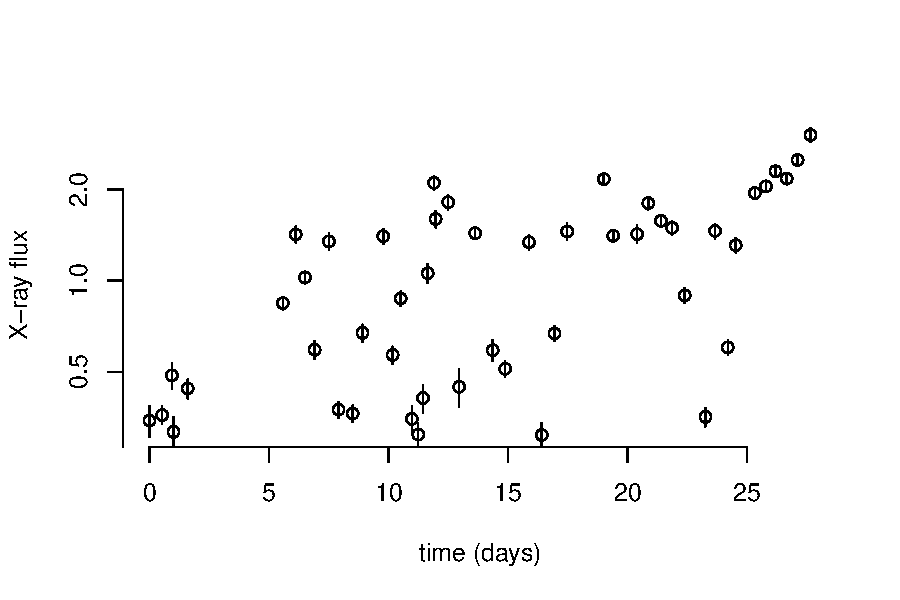
\includegraphics[width=\maxwidth]{figure/unnamed-chunk-3-1} 

}



\end{knitrout}

In this case all the elements of $x$ are independent and identically distributed (iid). They all have the same Gaussian distribution (with mean $\mu=0$ and variance $\sigma^2=1$), and they are independent, meaning that each point is drawn at random with no connection to any other point in the sequence.

We can think of these as $n=20$ draws of a scalar ($1$-dimensional) random variable. Or we could think of this as a single draw of a $n$-dimensional random vector, $\mathbf{x}$.\\
  
%%%%%%%%%%%%%%%%%%%%%%%%%%%%%%%%%%%%%%%%%%%%%
%%%%%%%%%%%%%%%%%%%%%%%%%%%%%%%%%%%%%%%%%%%%%%%
\vspace{0.4cm}
\textbf{The $n$-dimensional Gaussian distribution}\\

The $n$-dimensional Gaussian distribution has the following pdf

\begin{equation}
p(\mathbf{x}|\bmu, \Sigma) = \frac{1}{ (2 \pi)^{n/2} |\Sigma|^{1/2} } 
                 \exp \left( -\frac{1}{2} (\mathbf{x} - \bmu)^T
                 \Sigma^{-1} (\mathbf{x} - \bmu) \right)
\label{eqn:norm2}
\end{equation}
  
where $\mathbf{x}$ is an $n$-dimensional random vector, $\bmu$ is an $n$-dimensional vector of means and $\Sigma$ is an $n \times n$ matrix called the \emph{covariance matrix}. The (vector) mean $\bmu$ and covariance (matrix) $\Sigma$ completely specify a Gaussian distribution for any number of dimensions.

Like the 1-dimensional case (equation \ref{eqn:norm1}), the first term in equation \ref{eqn:norm2} ($1/([2 \pi ]^{n/2} |\Sigma|^{1/2} )$) is a normalisation term and ensures that
\begin{equation}
  \int_{-\infty}^{+\infty} p(\mathbf{x}) d\mathbf{x} = 1
\end{equation}
Inside the exponential is a \emph{quadratic form} 
\begin{equation}
 Q = (\mathbf{x} - \bmu)^T \Sigma^{-1} (\mathbf{x} - \bmu)
\end{equation}
which is the $n$-dimensional equivalent to the exponent in equation \ref{eqn:norm1} which we can write as $(x-\mu)(\sigma^2)^{-1}(x-\mu)$. 

A valid covariance matrix must have certain properties. It must be a square, symmetric matrix, $\Sigma_{ij} = \Sigma_{ji}$ for $i,j = 1, 2, \ldots, n$. It must be \emph{positive semi-definite}. This several things (most of which are equivalent to each other):
\begin{itemize}
\item Has a determinant $|\Sigma| \ge 0$
\item Has a unique Cholesky decomposition $\Sigma = LL^T$ where $L$ is a lower triangular matrix
\item Has an inverse $\Sigma^{-1}$ that is also positive semi-definite
\item Has quadratic form $\mathbf{y}^T \Sigma \mathbf{y} \ge 0$ and also $\mathbf{y}^T \Sigma^{-1} \mathbf{y} \ge 0$ for any real $n$-vector $\mathbf{y}$ (with equality only when $\mathbf{y} = \mathbf{0}$).
\item All the eigenvalues are $\lambda_i \ge 0$
\end{itemize}
Therefore $|\Sigma|^{-1/2}$ and $\Sigma^{-1}$ in equation \ref{eqn:norm2} are well-defined. An example is:

\begin{equation}
 \Sigma = \begin{pmatrix}
 1.00 & 0.50 & 0.10 & 0.01 \\
 0.50 & 1.50 & 0.40 & 0.10 \\
 0.10 & 0.40 & 2.00 & 0.30 \\
 0.01 & 0.10 & 0.30 & 3.00 
 \end{pmatrix}
\end{equation}

We can understand the information contained in $\Sigma$ as follows. The leading diagonal entires represent the variances of the elements of the random vector $\mathbf{x}$. I.e. $\Sigma_{ii} = \sigma_{i}^2$. The off-diagonal elements are the \emph{covariances} between the $i$th and $j$th elements, i.e. $cov(x_i, x_j) = \Sigma_{ij}$. These tell us if the $i$th and $j$th elements are well-correlated or not. If the covariances $\Sigma_{ij} = 0$ for $i \ne j$ then the value of $x_i$ is uncorrelated\footnote{In general, there is a difference between \emph{independent} and {uncorrelated}. However, in the special case of a Gaussian distribution they are equivalent.s} with $x_j$. The covariances must obey $|\Sigma_{ij}|^2 \le \Sigma_{ii} \Sigma_{jj}$. 

We can visualise this as an image using {\tt image(S)}. (Although this does require a few extra lines to `flip' the image so that the row $i=1$ appear at the top.)

\begin{knitrout}
\definecolor{shadecolor}{rgb}{0.969, 0.969, 0.969}\color{fgcolor}\begin{kframe}
\begin{alltt}
  \hlstd{S} \hlkwb{<-} \hlkwd{c}\hlstd{(}\hlnum{1.00}\hlstd{,} \hlnum{0.50}\hlstd{,} \hlnum{0.10}\hlstd{,} \hlnum{0.01}\hlstd{,}
         \hlnum{0.50}\hlstd{,} \hlnum{1.50}\hlstd{,} \hlnum{0.40}\hlstd{,} \hlnum{0.10}\hlstd{,}
         \hlnum{0.10} \hlstd{,}\hlnum{0.40} \hlstd{,}\hlnum{2.00} \hlstd{,}\hlnum{0.30}\hlstd{,}
         \hlnum{0.01}\hlstd{,} \hlnum{0.10}\hlstd{,} \hlnum{0.30}\hlstd{,} \hlnum{3.00}\hlstd{)}
\hlstd{S} \hlkwb{<-} \hlkwd{matrix}\hlstd{(S,} \hlkwc{nrow}\hlstd{=}\hlnum{4}\hlstd{)}
\hlkwd{image}\hlstd{(}\hlkwc{x}\hlstd{=}\hlnum{1}\hlopt{:}\hlnum{4}\hlstd{,} \hlkwc{y}\hlstd{=}\hlnum{1}\hlopt{:}\hlnum{4}\hlstd{,} \hlkwc{z}\hlstd{=}\hlkwd{sqrt}\hlstd{(S[}\hlnum{1}\hlopt{:}\hlnum{4}\hlstd{,}\hlnum{4}\hlopt{:}\hlnum{1}\hlstd{]),}
      \hlkwc{xlab}\hlstd{=}\hlstr{""}\hlstd{,} \hlkwc{ylab}\hlstd{=}\hlstr{""}\hlstd{,} \hlkwc{bty} \hlstd{=} \hlstr{"n"}\hlstd{,} \hlkwc{asp}\hlstd{=}\hlnum{1}\hlstd{,}
      \hlkwc{cex.axis}\hlstd{=}\hlnum{1.4}\hlstd{,} \hlkwc{xaxt}\hlstd{=}\hlstr{"n"}\hlstd{,} \hlkwc{yaxt}\hlstd{=}\hlstr{"n"}\hlstd{)}
\hlkwd{axis}\hlstd{(}\hlnum{3}\hlstd{,} \hlkwc{at} \hlstd{=} \hlnum{1}\hlopt{:}\hlnum{4}\hlstd{,} \hlkwc{cex.axis}\hlstd{=}\hlnum{1.4}\hlstd{)}
\hlkwd{axis}\hlstd{(}\hlnum{2}\hlstd{,} \hlkwc{at} \hlstd{=} \hlnum{1}\hlopt{:}\hlnum{4}\hlstd{,} \hlkwc{pos} \hlstd{=} \hlnum{0.5}\hlstd{,} \hlkwc{labels}\hlstd{=}\hlkwd{c}\hlstd{(}\hlstr{"4"}\hlstd{,}\hlstr{"3"}\hlstd{,}\hlstr{"2"}\hlstd{,}\hlstr{"1"}\hlstd{),} \hlkwc{cex.axis}\hlstd{=}\hlnum{1.4}\hlstd{)}
\end{alltt}
\end{kframe}

{\centering 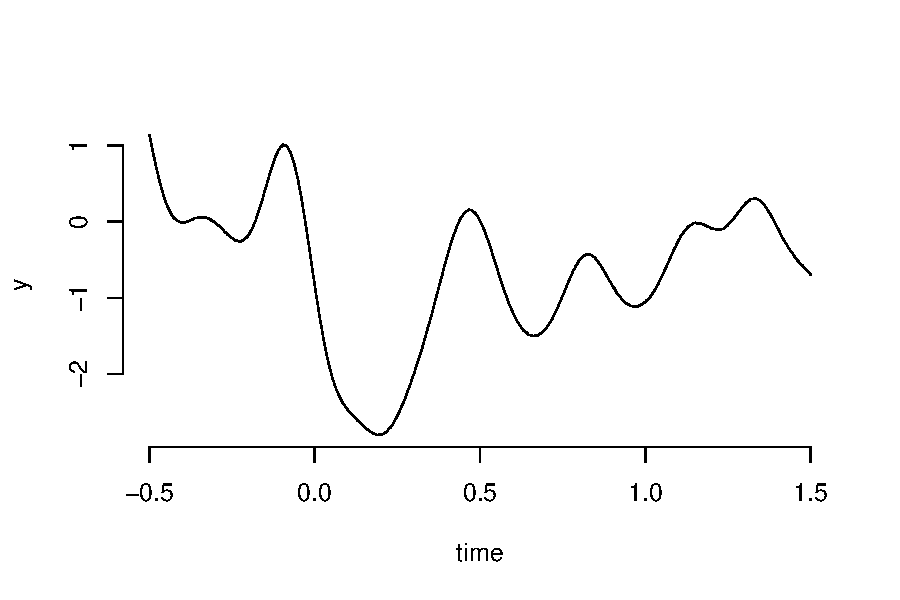
\includegraphics[width=\maxwidth]{figure/unnamed-chunk-4-1} 

}



\end{knitrout}

What is covariance? Let's start with the mean, which describes the `centre' of the distribution of the random variable
\begin{equation}
  \mu = E[x] = \int_{-\infty}^{+\infty} x p(x) dx.
\end{equation}
This is the definition of the \emph{mean} or \emph{expectation} of a single variable. The same applies to vectors.
\begin{equation}
  \bmu = E[\mathbf{x}] = \int_{-\infty}^{+\infty} \mathbf{x} p(\mathbf{x}) d\mathbf{x}.
\end{equation}
The variance is the expectation of the \emph{square deviation} around the mean
\begin{equation}
  \sigma_x^2 = E[(x-\mu)(x-\mu)],
\end{equation}
it describes the typical spread around the mean. If we have many variables ($x_i$, $x_j$, etc.), we need to know not just how each one is spread but whether each one varies in a way that is correlated with any other variables. The covariance tells us how $x_i$ and $x_j$ vary together
\begin{equation}
  \Sigma_{ij} = E[(x_i-\mu_i)(x_j-\mu_j)]
\end{equation}
So you can see
\begin{equation}
  \Sigma_{ii} = E[(x_i-\mu_i)(x_i-\mu_i)] = \sigma_{i}^2
\end{equation}
Informally, you can think about it this way. If $x_j$ is often above its mean when $x_i$ is also above its mean (and $x_j$ is below usually when $x_i$ is below), then the product $(x_i-\mu_i)(x_j-\mu_j)$ is likely to be positive, and positive in expectation. So there will be positive covariance. If $x_j$ is independent of $x_i$, so that it is equally likely to be above or below its mean when $x_i$ is above its mean, then $(x_i-\mu_i)(x_j-\mu_j)$ is equally likely to be positive or negative, so will tend to zero in expectation. In this case the covariance is zero. So it tells us how much two variables, or two elements of a random vector, vary together.\\

%%%%%%%%%%%%%%%%%%%%%%%%%%%%%%%%%%%%%%%%%%%%%%%
\vspace{0.4cm}
\textbf{Generating $n$-dimensional random vectors}\\

To generate an $n$-dimensional Gaussian random vector we first define a vector of $n$ means, and an $n \times n$ covariance matrix. We will first begin with the identity matrix $I_n$.

\begin{knitrout}
\definecolor{shadecolor}{rgb}{0.969, 0.969, 0.969}\color{fgcolor}\begin{kframe}
\begin{alltt}
  \hlstd{mu} \hlkwb{<-} \hlkwd{array}\hlstd{(}\hlnum{0}\hlstd{,} \hlkwc{dim} \hlstd{= n)}
  \hlstd{S} \hlkwb{<-} \hlkwd{diag}\hlstd{(n)}
  \hlkwd{print}\hlstd{(S[}\hlnum{1}\hlopt{:}\hlnum{6}\hlstd{,} \hlnum{1}\hlopt{:}\hlnum{6}\hlstd{])}
\end{alltt}
\begin{verbatim}
##      [,1] [,2] [,3] [,4] [,5] [,6]
## [1,]    1    0    0    0    0    0
## [2,]    0    1    0    0    0    0
## [3,]    0    0    1    0    0    0
## [4,]    0    0    0    1    0    0
## [5,]    0    0    0    0    1    0
## [6,]    0    0    0    0    0    1
\end{verbatim}
\end{kframe}
\end{knitrout}

Now we need to load an extra \emph{package} which contains the function we need

\begin{knitrout}
\definecolor{shadecolor}{rgb}{0.969, 0.969, 0.969}\color{fgcolor}\begin{kframe}
\begin{alltt}
  \hlkwd{install.packages}\hlstd{(}\hlstr{"mvtnorm"}\hlstd{)}
\end{alltt}
\end{kframe}
\end{knitrout}

Once this is installed we never need to do this again. 
Now we have access to a new function rmvnorm.

\begin{knitrout}
\definecolor{shadecolor}{rgb}{0.969, 0.969, 0.969}\color{fgcolor}\begin{kframe}
\begin{alltt}
  \hlstd{x} \hlkwb{<-} \hlstd{mvtnorm}\hlopt{::}\hlkwd{rmvnorm}\hlstd{(}\hlnum{1}\hlstd{, mu, S)}
  \hlkwd{plot}\hlstd{(x[}\hlnum{1}\hlopt{:}\hlstd{n])}
\end{alltt}
\end{kframe}

{\centering 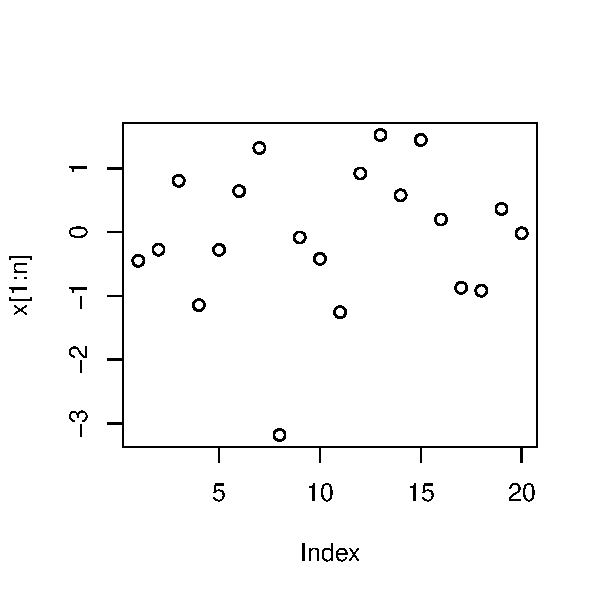
\includegraphics[width=\maxwidth]{figure/unnamed-chunk-7-1} 

}



\end{knitrout}

The output of {\tt rmvnorm} is a $1 \times n$ array. In order to plot the 20 value, the simplest method is to use {\tt [1:n]} to extract the elements $1$ to $n$. Notice there is no \emph{structure} to the output data, again the values are all indepenent of one another.\\

\textbf{Changing the covariance matrix}\\

Now, let's introduce more structure to the data, by using a less trivial covariance matrix. We first define positions along the horizontal axis by a vector $\mathbf{t}$. This might be as simple as $\mathbf{t} = \{1, 2, \ldots, n\}$ but the spacing could be arbitrary, $\mathbf{t} = \{ t_i | i=1,2,\ldots,n\}$.

We define the \emph{lag} as the separation (in time) between two points, $\tau_{ij} = t_i - t_j$. And the absolute value of this is $r = |\tau|$. The \emph{autocovariance function} (ACV) defines the variances and covariances for each element of a random vector $\mathbf{y}$ as a function of $r$. 
\begin{equation}
ACV(r) = A \exp \left( - \frac{r^2}{2l^2} \right) 
\label{eqn:acv1}
\end{equation}
or equivalently 
\begin{equation}
ACV(|t_i - t_j|) = A \exp \left( - \frac{1}{2}\frac{|t_i-t_j|^2}{l^2} \right)
\label{eqn:acv2}
\end{equation}
First, let's plot this for two different $l$ values. We define a function 
\begin{knitrout}
\definecolor{shadecolor}{rgb}{0.969, 0.969, 0.969}\color{fgcolor}\begin{kframe}
\begin{alltt}
\hlcom{#define a function to compute the simple ACV}
\hlstd{acv} \hlkwb{<-} \hlkwa{function}\hlstd{(}\hlkwc{tau}\hlstd{,} \hlkwc{A}\hlstd{,} \hlkwc{l}\hlstd{) \{}
  \hlstd{acov} \hlkwb{<-} \hlstd{A}\hlopt{*}\hlkwd{exp}\hlstd{(}\hlopt{-}\hlnum{0.5}\hlopt{*}\hlstd{(tau}\hlopt{/}\hlstd{l)}\hlopt{^}\hlnum{2}\hlstd{)}
  \hlkwd{return}\hlstd{(acov)}
\hlstd{\}}
\end{alltt}
\end{kframe}
\end{knitrout}

Now we can use this to compute an ACV when we need it.

\begin{knitrout}
\definecolor{shadecolor}{rgb}{0.969, 0.969, 0.969}\color{fgcolor}\begin{kframe}
\begin{alltt}
\hlstd{A} \hlkwb{<-} \hlnum{1.0}   \hlcom{# set the amplitude parameter}
\hlstd{l} \hlkwb{<-} \hlnum{3.0}   \hlcom{# set the scale parameter}
\hlstd{tau} \hlkwb{<-} \hlkwd{seq}\hlstd{(}\hlopt{-}\hlnum{25}\hlstd{,} \hlnum{25}\hlstd{,} \hlkwc{by} \hlstd{=} \hlnum{0.25}\hlstd{)} \hlcom{# define lags}
\hlstd{y} \hlkwb{<-} \hlkwd{acv}\hlstd{(tau, A, l)}            \hlcom{# compute ACV}
\hlkwd{plot}\hlstd{(tau, y,} \hlkwc{type} \hlstd{=} \hlstr{"l"}\hlstd{)}       \hlcom{# plot the result}
\hlstd{l} \hlkwb{<-} \hlnum{0.75}                      \hlcom{# change the scale}
\hlstd{y.2} \hlkwb{<-} \hlkwd{acv}\hlstd{(tau, A, l)}          \hlcom{# re-compute the ACV}
\hlkwd{lines}\hlstd{(tau, y.2,} \hlkwc{col} \hlstd{=} \hlstr{"blue"}\hlstd{)}  \hlcom{# overlay the new curve}
\end{alltt}
\end{kframe}

{\centering 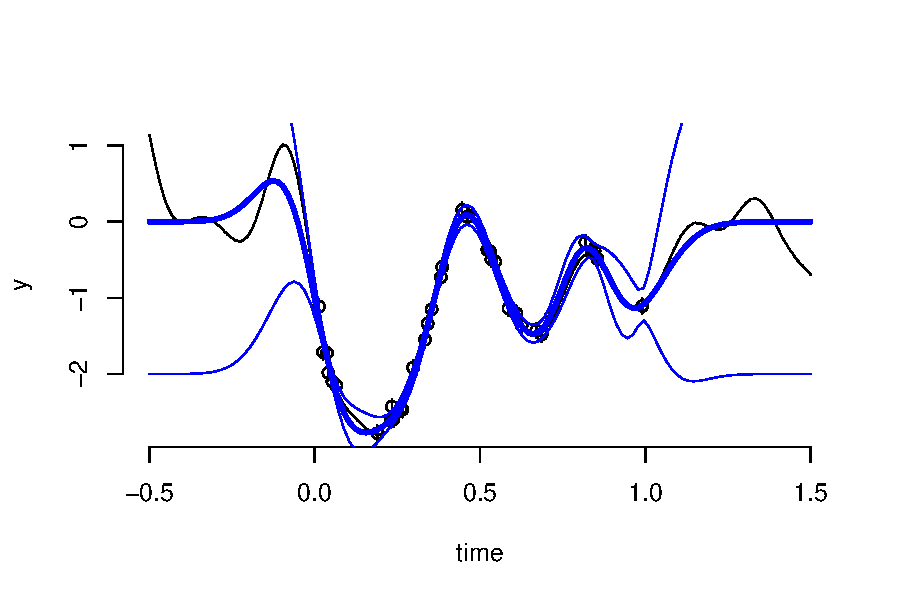
\includegraphics[width=\maxwidth]{figure/unnamed-chunk-9-1} 

}



\end{knitrout}

Now let's define a vector of times $\mathbf{t} = \{t_1, t_2, \ldots, t_M\}$.

\begin{knitrout}
\definecolor{shadecolor}{rgb}{0.969, 0.969, 0.969}\color{fgcolor}\begin{kframe}
\begin{alltt}
 \hlstd{t} \hlkwb{<-} \hlkwd{c}\hlstd{(}\hlnum{1}\hlstd{,} \hlnum{2}\hlstd{,} \hlnum{4}\hlstd{,} \hlnum{7.5}\hlstd{,} \hlnum{8.0}\hlstd{,} \hlnum{8.5}\hlstd{,} \hlnum{9}\hlstd{,} \hlnum{10}\hlstd{)}
\end{alltt}
\end{kframe}
\end{knitrout}

We want to compute the covariance matrix using the autocovariance function (equation \ref{eqn:acv2}) and the list of times. We first make a matrix of all the time differences $\tau_{ij} = |t_i - t_j|$

\begin{knitrout}
\definecolor{shadecolor}{rgb}{0.969, 0.969, 0.969}\color{fgcolor}\begin{kframe}
\begin{alltt}
  \hlstd{tau} \hlkwb{<-} \hlkwd{outer}\hlstd{(t, t,} \hlstr{"-"}\hlstd{)}
  \hlstd{tau} \hlkwb{<-} \hlkwd{abs}\hlstd{(tau)}
  \hlkwd{print}\hlstd{(tau)}
\end{alltt}
\begin{verbatim}
##      [,1] [,2] [,3] [,4] [,5] [,6] [,7] [,8]
## [1,]  0.0  1.0  3.0  6.5  7.0  7.5  8.0  9.0
## [2,]  1.0  0.0  2.0  5.5  6.0  6.5  7.0  8.0
## [3,]  3.0  2.0  0.0  3.5  4.0  4.5  5.0  6.0
## [4,]  6.5  5.5  3.5  0.0  0.5  1.0  1.5  2.5
## [5,]  7.0  6.0  4.0  0.5  0.0  0.5  1.0  2.0
## [6,]  7.5  6.5  4.5  1.0  0.5  0.0  0.5  1.5
## [7,]  8.0  7.0  5.0  1.5  1.0  0.5  0.0  1.0
## [8,]  9.0  8.0  6.0  2.5  2.0  1.5  1.0  0.0
\end{verbatim}
\end{kframe}
\end{knitrout}

The R function {\tt outer()} is very useful. It takes two vectors $\{x_i\}$ and $\{y_i\}$ and an operation and computes the operation for every pair of values. In this case the operation is simply ``-'' so it subtracts all the $t_j$ from all the $t_i$ and arranges the output in a matrix, i.e. $\tau_{ij} = |t_i - t_j|$.

Now we can use our function {\tt acv()} defined above to compute the ACV for every value of $\tau_{ij}$ in the matrix. This works because the function {\tt acv()} will accept a matrix as input, i.e. $S_{ij} = ACV(\tau_{ij})$.

\begin{knitrout}
\definecolor{shadecolor}{rgb}{0.969, 0.969, 0.969}\color{fgcolor}\begin{kframe}
\begin{alltt}
  \hlstd{S} \hlkwb{<-} \hlkwd{acv}\hlstd{(tau,} \hlnum{1.0}\hlstd{,} \hlnum{2}\hlstd{)}
  \hlkwd{print}\hlstd{(}\hlkwd{signif}\hlstd{(S[}\hlnum{1}\hlopt{:}\hlnum{5}\hlstd{,}\hlnum{1}\hlopt{:}\hlnum{5}\hlstd{],} \hlnum{3}\hlstd{))}   \hlcom{# print only to 3 signif. fig.}
\end{alltt}
\begin{verbatim}
##         [,1]   [,2]  [,3]    [,4]    [,5]
## [1,] 1.00000 0.8820 0.325 0.00509 0.00219
## [2,] 0.88200 1.0000 0.607 0.02280 0.01110
## [3,] 0.32500 0.6070 1.000 0.21600 0.13500
## [4,] 0.00509 0.0228 0.216 1.00000 0.96900
## [5,] 0.00219 0.0111 0.135 0.96900 1.00000
\end{verbatim}
\end{kframe}
\end{knitrout}

Now we can use this to compute a new Gaussian vector 

\begin{knitrout}
\definecolor{shadecolor}{rgb}{0.969, 0.969, 0.969}\color{fgcolor}\begin{kframe}
\begin{alltt}
  \hlstd{M} \hlkwb{<-} \hlkwd{length}\hlstd{(t)}                  \hlcom{# how many elements in the vector?}
  \hlstd{mu} \hlkwb{<-} \hlkwd{array}\hlstd{(}\hlnum{0}\hlstd{,} \hlkwc{dim}\hlstd{=M)}           \hlcom{# set all means to zero}
  \hlstd{y} \hlkwb{<-} \hlstd{mvtnorm}\hlopt{::}\hlkwd{rmvnorm}\hlstd{(}\hlnum{1}\hlstd{, mu, S)} \hlcom{# generate random vector}
  \hlkwd{plot}\hlstd{(t, y[}\hlnum{1}\hlopt{:}\hlstd{M])}
\end{alltt}
\end{kframe}

{\centering 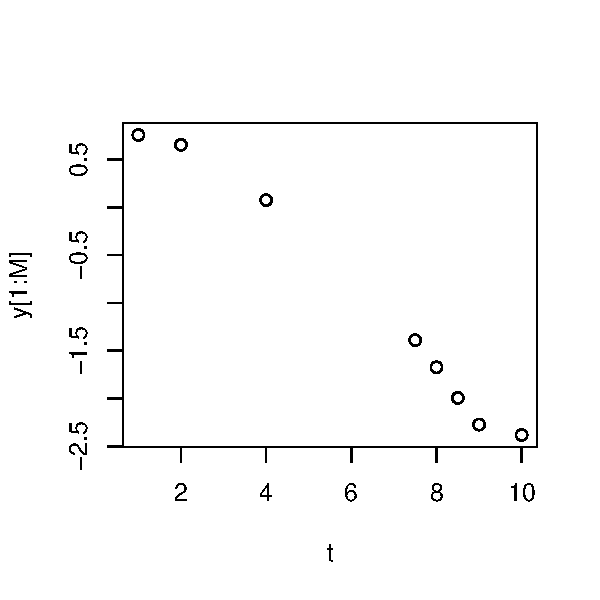
\includegraphics[width=\maxwidth]{figure/unnamed-chunk-13-1} 

}



\end{knitrout}

There is a more structure in these data. We can see this more easily if we evalute many more points. However, we may start to see numerical problems. If you repeat the above steps but first set

\begin{knitrout}
\definecolor{shadecolor}{rgb}{0.969, 0.969, 0.969}\color{fgcolor}\begin{kframe}
\begin{alltt}
    \hlstd{t} \hlkwb{<-} \hlkwd{seq}\hlstd{(}\hlnum{0}\hlstd{,} \hlnum{10}\hlstd{,} \hlkwc{by} \hlstd{=} \hlnum{0.2}\hlstd{)}
\end{alltt}
\end{kframe}
\end{knitrout}

so that $\mathbf{t} = \{0, 0.2, 0.4, \ldots, 9.8, 10.0\}$ you may find that {\tt rmvnorm()} fails to run. For example

\begin{knitrout}
\definecolor{shadecolor}{rgb}{0.969, 0.969, 0.969}\color{fgcolor}\begin{kframe}
\begin{alltt}
  \hlstd{t} \hlkwb{<-} \hlkwd{seq}\hlstd{(}\hlnum{0}\hlstd{,}\hlnum{10}\hlstd{,}\hlkwc{by}\hlstd{=}\hlnum{0.2}\hlstd{)}
  \hlstd{M} \hlkwb{<-} \hlkwd{length}\hlstd{(t)}           \hlcom{# how many elements in the vector?}
  \hlstd{mu} \hlkwb{<-} \hlkwd{array}\hlstd{(}\hlnum{0}\hlstd{,} \hlkwc{dim}\hlstd{=M)}    \hlcom{# set all means to zero}
  \hlstd{tau} \hlkwb{<-} \hlkwd{outer}\hlstd{(t, t,} \hlstr{"-"}\hlstd{)}
  \hlstd{tau} \hlkwb{<-} \hlkwd{abs}\hlstd{(tau)}
  \hlstd{S} \hlkwb{<-} \hlkwd{acv}\hlstd{(tau,} \hlnum{1.0}\hlstd{,} \hlnum{1}\hlstd{)}
  \hlstd{y} \hlkwb{<-} \hlstd{mvtnorm}\hlopt{::}\hlkwd{rmvnorm}\hlstd{(}\hlnum{1}\hlstd{, mu, S)}   \hlcom{# generate a new, random vector}
\end{alltt}


{\ttfamily\noindent\color{warningcolor}{\#\# Warning in sqrt(ev\$values): NaNs produced}}\end{kframe}
\end{knitrout}

The matrix $S$ that we made is not quite right. This because we are computing with a $51 \times 51$ matrix. Tiny numerical errors when computing or storing the matrix could mean it is not quite positive definite (so $\det S \le 0$). 

But in R we can add new matrix functions which allow us to fix these issues, and force $S$ to be positive definite. We need a new package called {\tt Matrix}. You may need to install it on your computer before you can use it.

\begin{knitrout}
\definecolor{shadecolor}{rgb}{0.969, 0.969, 0.969}\color{fgcolor}\begin{kframe}
\begin{alltt}
  \hlkwd{install.packages}\hlstd{(}\hlstr{"Matrix"}\hlstd{)}
\end{alltt}
\end{kframe}
\end{knitrout}

Now we can use a function called {\tt nearPD()} to find the nearest positive definite matrix. If you read the instructions ({\tt ? Matrix::nearPD}) you will find the output is not in a simple matrix formal. So we need some extra lines to handle this, and convert it to a normal {\tt matrix} object.
  
\begin{knitrout}
\definecolor{shadecolor}{rgb}{0.969, 0.969, 0.969}\color{fgcolor}\begin{kframe}
\begin{alltt}
\hlstd{pd} \hlkwb{<-} \hlstd{Matrix}\hlopt{::}\hlkwd{nearPD}\hlstd{(S)}
\hlkwa{if} \hlstd{(pd}\hlopt{$}\hlstd{converged} \hlopt{==} \hlnum{FALSE}\hlstd{) \{}
  \hlkwd{stop}\hlstd{(}\hlstr{'near PD failed to converge'}\hlstd{)}
\hlstd{\}}
\hlstd{S} \hlkwb{<-} \hlkwd{matrix}\hlstd{(pd}\hlopt{$}\hlstd{mat,} \hlkwc{nrow} \hlstd{= M)}
\end{alltt}
\end{kframe}
\end{knitrout}

Now we have a positive definite $S$ we can run {\tt rmvnorm()} as before.

\begin{knitrout}
\definecolor{shadecolor}{rgb}{0.969, 0.969, 0.969}\color{fgcolor}\begin{kframe}
\begin{alltt}
  \hlstd{y} \hlkwb{<-} \hlstd{mvtnorm}\hlopt{::}\hlkwd{rmvnorm}\hlstd{(}\hlnum{1}\hlstd{, mu, S)}   \hlcom{# generate a new, random vector}
  \hlkwd{plot}\hlstd{(t, y[}\hlnum{1}\hlopt{:}\hlstd{M],} \hlkwc{type} \hlstd{=} \hlstr{"l"}\hlstd{)}
\end{alltt}
\end{kframe}

{\centering 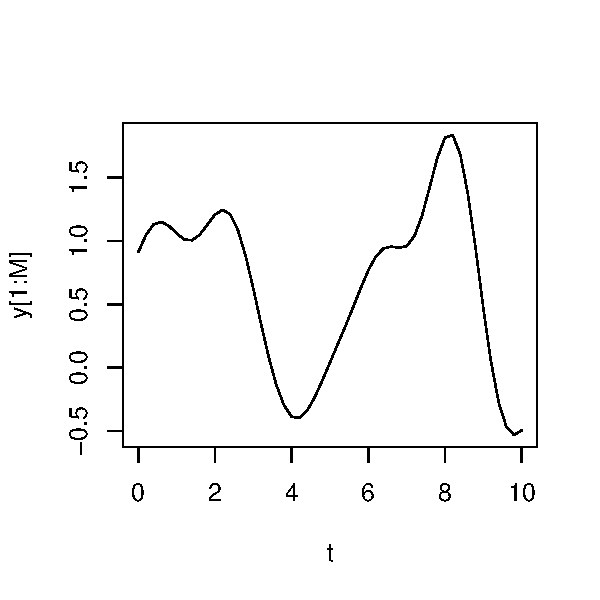
\includegraphics[width=\maxwidth]{figure/unnamed-chunk-18-1} 

}



\end{knitrout}

And we can re-run with more points if needed and it should still work. Although as $M>1000$ and the $S$ matrix gets very large ($10^3 \times 10^3$) we may find the numerical stability becomes a problem again.

Now, let's generate several vector outputs using a simple loop

\begin{knitrout}
\definecolor{shadecolor}{rgb}{0.969, 0.969, 0.969}\color{fgcolor}\begin{kframe}
\begin{alltt}
  \hlkwd{plot}\hlstd{(}\hlnum{0}\hlstd{,} \hlnum{0}\hlstd{,} \hlkwc{type} \hlstd{=} \hlstr{"n"}\hlstd{,} \hlkwc{xlim} \hlstd{=} \hlkwd{c}\hlstd{(}\hlnum{0}\hlstd{,} \hlnum{10}\hlstd{),} \hlkwc{ylim} \hlstd{=} \hlkwd{c}\hlstd{(}\hlopt{-}\hlnum{3}\hlstd{,} \hlnum{3}\hlstd{),}
       \hlkwc{xlab} \hlstd{=} \hlstr{"time"}\hlstd{,} \hlkwc{ylab} \hlstd{=} \hlstr{"y(t)"}\hlstd{)}  \hlcom{# open blank plot}
  \hlkwa{for} \hlstd{(i} \hlkwa{in} \hlnum{1}\hlopt{:}\hlnum{10}\hlstd{) \{}
    \hlstd{y} \hlkwb{<-} \hlstd{mvtnorm}\hlopt{::}\hlkwd{rmvnorm}\hlstd{(}\hlnum{1}\hlstd{, mu, S)}   \hlcom{# generate a new, random vector}
    \hlkwd{lines}\hlstd{(t, y[}\hlnum{1}\hlopt{:}\hlstd{M],} \hlkwc{lwd} \hlstd{=} \hlnum{2}\hlstd{,} \hlkwc{col} \hlstd{=} \hlkwd{rainbow}\hlstd{(}\hlnum{10}\hlstd{)[i])}
  \hlstd{\}}
\end{alltt}
\end{kframe}\begin{figure}

{\centering 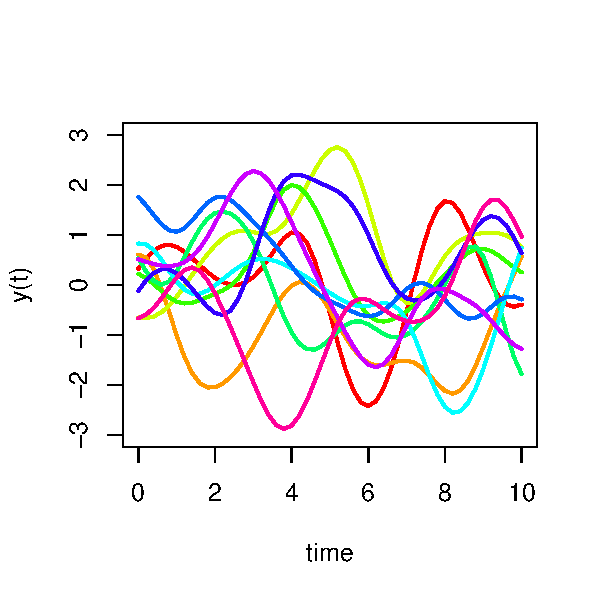
\includegraphics[width=\maxwidth]{figure/unnamed-chunk-19-1} 

}

\caption[Example GP output with ]{Example GP output with $l=1$}\label{fig:unnamed-chunk-19}
\end{figure}


\end{knitrout}

The figures show what happens when we repeat the above for $l=0.2$ and  $l=5$. 

\begin{knitrout}
\definecolor{shadecolor}{rgb}{0.969, 0.969, 0.969}\color{fgcolor}\begin{figure}

{\centering 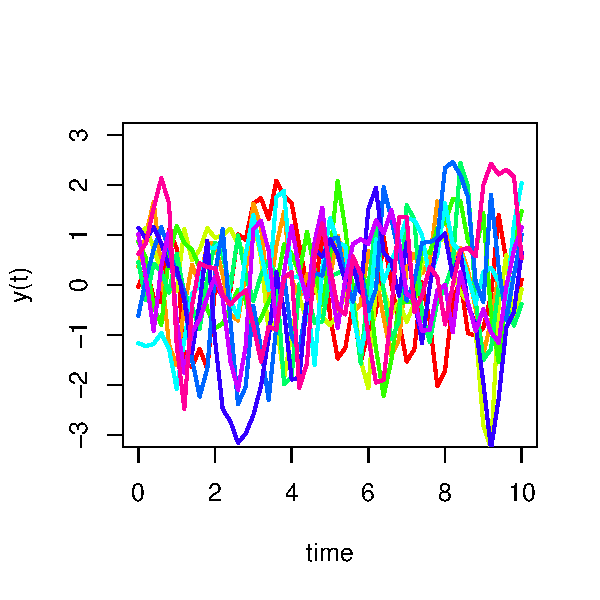
\includegraphics[width=\maxwidth]{figure/unnamed-chunk-20-1} 

}

\caption[Example GP outputwith ]{Example GP outputwith $l=0.2$}\label{fig:unnamed-chunk-20}
\end{figure}


\end{knitrout}

\begin{knitrout}
\definecolor{shadecolor}{rgb}{0.969, 0.969, 0.969}\color{fgcolor}\begin{figure}

{\centering 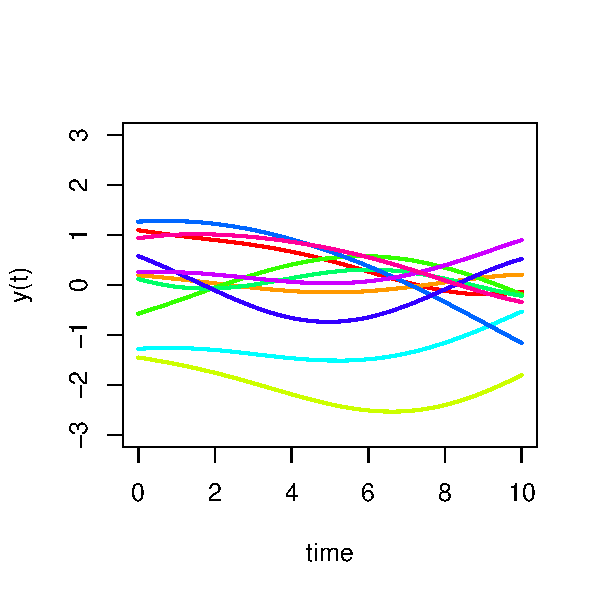
\includegraphics[width=\maxwidth]{figure/unnamed-chunk-21-1} 

}

\caption[Example GP output with ]{Example GP output with $l=5$}\label{fig:unnamed-chunk-21}
\end{figure}


\end{knitrout}

There may be better ways to fix the numerical issues that arise when $M$ becomes large. This would be good to study. 

\end{document}

